\documentclass[12pt]{article}

\usepackage[letterpaper, margin=1in]{geometry}
\usepackage{amsmath, amssymb, mathrsfs}
\usepackage{graphicx}

\title{DFTnet: efficiently training large neural networks}
\author{Liu Jiacheng}

\begin{document}

\maketitle

\section{Alternative Dense Layer}

In a canonical dense layer in neural network, suppose its input size is $p$ and output size is $q$, then it is described by matrix
\begin{align*}
	\begin{bmatrix}
		w_{11} & w_{12} & \hdots & w_{1p} \\
		w_{21} & w_{22} & \hdots & w_{2p} \\
		\vdots & \vdots & \ddots & \vdots \\
		w_{q1} & w_{q2} & \hdots & w_{qp}
	\end{bmatrix}
\end{align*}
the forward propagation is
\begin{align*}
	Z &= W A
\end{align*}
and the back propagation is
\begin{align*}
	dW &= \frac{\partial{J}}{\partial{W}} = \frac{1}{m} dZ A^T \\
	dA &= \frac{\partial{J}}{\partial{A}} = W^T dZ
\end{align*}

Now assume $p=q=n$ (we will consider $p \neq q$ later). If the weight matrix $W$ has form
\begin{align*}
	\begin{bmatrix}
		w_1 & w_2 & \hdots & w_n \\
		w_2 & w_3 & \hdots & w_1 \\
		\vdots & \vdots & \ddots & \vdots \\
		w_n & w_1 & \hdots & w_{n-1}
	\end{bmatrix}
\end{align*}
Then we would conveniently have (see derivation below) forward propagation
\begin{align*}
	Z &= w * A = \mathscr{F}^{-1}(\mathscr{F}(w) \mathscr{F}(A))
\end{align*}
and back propagation
\begin{align*}
	dw &= \mathscr{F}(\frac{1}{m} \mathscr{F}^{-1}(dZ) \mathscr{F}(A)) \\
	dA &= \mathscr{F}(\mathscr{F}^{-1}(dZ) \mathscr{F}(w))
\end{align*}
where $*$ is linear convolution and $w = \begin{bmatrix} w_1 & w_2 & \hdots & w_n \end{bmatrix}^T$. 

\section{I/O Size Mismatch}

If $p \neq q$, let $n = \max{(p,q)}$, the weight matrix should be 
\begin{align*}
	\begin{bmatrix}
		w_1 & w_2 & \hdots & w_p \\
		w_2 & w_3 & \hdots & w_{(p+1)\%n} \\
		\vdots & \vdots & \ddots & \vdots \\
		w_q & w_{(q+1)\%n} & \hdots & w_{(p+q-1)\%n}
	\end{bmatrix}
\end{align*}
In this case, we can still perform DFT by making the following changes: 
\begin{itemize}
\item Before DFT, pad the input vector with zeros to the end, up to size $n$. 
\item After DFT, truncate the output vector from the end, down to size $q$. 
\end{itemize}
It can be proved that this is equivalent to simple convolution with mismatched I/O size. 

\section{Time Complexity}

Let $n = \max{(p,q)}$. For each dense layer, the cost of forward propagation is $\Theta(3n\log{n} + n)$ and the cost of back propagation is $\Theta(3n\log{n} + 2n)$. This is significantly lower than the $\Theta(pq)$ complexity in canonical dense layer. This implies that we can build wider dense layers given that we reuse the weights circularly. 

\section{Derivation}

\begin{align*}
	\mathscr{F}(A) &= DFT(A) \\
	\mathscr{F}(w) &= DFT(w) \\
	\mathscr{F}(Z) &= \mathscr{F}(w) \mathscr{F}(A) \\
	Z &= DFT^{-1}(\mathscr{F}(Z))
\end{align*}
\begin{align*}
	d\mathscr{F}(Z) &= \frac{\partial{J}}{\partial{\mathscr{F}(Z)}} = DFT^{-1}(dZ) = \mathscr{F}^{-1}(dZ) \\
	d\mathscr{F}(w) &= \frac{\partial{J}}{\partial{\mathscr{F}(w)}} = \frac{1}{m} d\mathscr{F}(Z) \mathscr{F}(A) \\
	d\mathscr{F}(A) &= \frac{\partial{J}}{\partial{\mathscr{F}(A)}} = d\mathscr{F}(Z) \mathscr{F}(w) \\
	dw &= \frac{\partial{J}}{\partial{w}} = DFT(d\mathscr{F}(w)) = \mathscr{F}(d\mathscr{F}(w)) = \mathscr{F}(\frac{1}{m} \mathscr{F}^{-1}(dZ) \mathscr{F}(A)) \\
	dA &= \frac{\partial{J}}{\partial{A}} = DFT(d\mathscr{F}(A)) = \mathscr{F}(d\mathscr{F}(A)) = \mathscr{F}(\mathscr{F}^{-1}(dZ) \mathscr{F}(w))
\end{align*}

\section{Experiment}

I trained a DFTnet: a neural network composed purely by DFT dense layers and ReLU activation. It has layer width $785, 4096, 1024, 256, 64, 10$. The model is fit into MNIST dataset and the result is comparable to a canonical neural network. 
\begin{figure}[h]
	\centering
	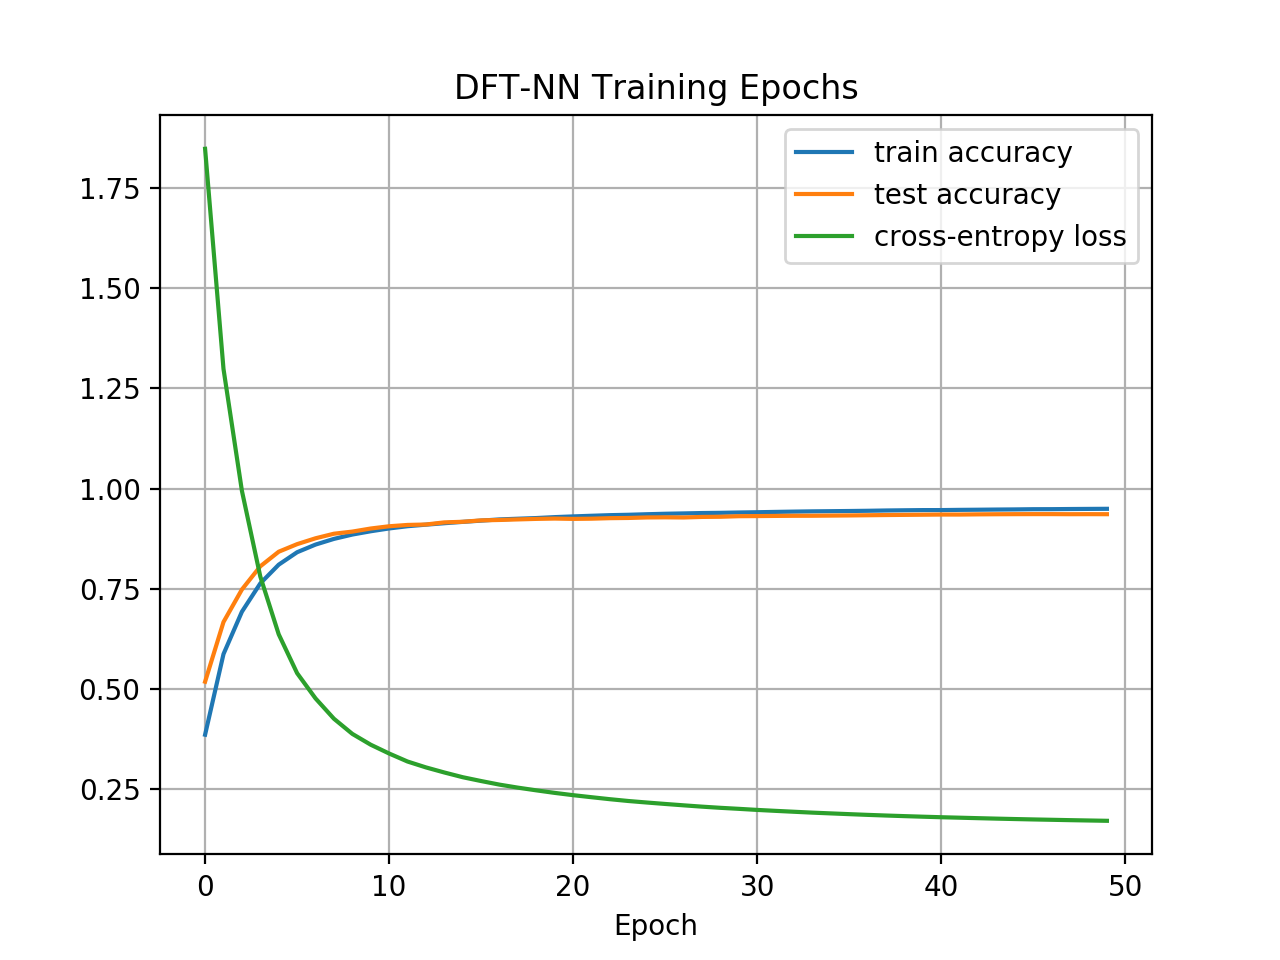
\includegraphics[scale=0.8]{fig.png}
\end{figure}

% fast computation for batches (like n3 to nlog7?)
% DFT-1 - relu - DFT optimization

\end{document}
